%%%% ijcai11.tex

\typeout{IJCAI-13 Instructions for Authors}

% These are the instructions for authors for IJCAI-13.
% They are the same as the ones for IJCAI-11 with superficical wording
%   changes only.

\documentclass{article}
% The file ijcai13.sty is the style file for IJCAI-13 (same as ijcai07.sty).
\usepackage{ijcai13}
\usepackage{graphicx}
\usepackage{algorithmic}
\usepackage{algorithm}
% Adaptation au français
\usepackage[utf8]{inputenc}

% Use the postscript times font!
\usepackage{times}

\usepackage{enumitem}
% Permet d'afficher un espace après le logo Latex, compliqué sinon
\usepackage{xspace}


\title{Rapport de projet}
\author{Théo Q, Corto C, Brandon FL \\
Université de Nice\\
France}

\begin{document}

\maketitle


\begin{abstract}
Dans ce projet nous étudions l'impact de la proportion de fourmis chercheuse et ramasseuses dans une fourmilière sur la récolte de nourriture. Nous utilisons pour cela un algorithme de type "Ant Colony Optimization (ACO)" écrit en Netlogo. Notre modèle utilise deux types de fourmis : ramasseuse et chercheuses déposant chacunes des phéromones spécifiques et des tas de nourritures à éloignement du nid variable. En faisant varier la répartition des fourmis dans la fourmilière lors de multiples simulations nous avons produits des données expérimentales . Celles-ci étés  étudiés avec le logiciel R pour extraire un modèle mathématique. Finalement l'analyse de la fonction modélisant le temps de récupération de toutes la nourriture en fonction du pourcentage de chercheuse dans la population présente un minimum local en 67,18\% ce qui s'approche des observations faites dans la nature.
\end{abstract}
\section{Introduction}
\subsection{Contexte}
Les "Algorithmes de colonies de fourmis" forment une catégorie d'algorithmes d'optimisation basés sur la modélisation d'une colonie de fourmis. En effet bien qu'ayant des capacités individuelles limités ces insectes arrivent collectivement à des solution optimales de problèmes complexes. 



Dans le cadre de l'UE "Projet Scientifique Informatique nous avons choisi le sujet "Colonie de fourmis" d'étude parmi de nombreux proposés. Le modèle de base contenait un seul type de fourmis et trois tas de nourritures fixes. Nous l'avons alors perfectionné.
\subsection{Etat de l'art}
L'ACO est de plus en plus utilisé aujourd'hui dans de très nombreux domaines. Plus particulièrement dans les domaines suivants : planification, routage réseau, affectation, ensembles, conception de circuit nanoélectroniques, traitement d'image etc. Tout les problèmes pouvant se ramener a la recherche d'un chemin optimal dans un graphe en général.
\subsection{Questions scientifiques}
\section{Modélisation}
Pour notre projet nous avons réalisé une simulation via l'outils NetLogo. NetLogo étant un programme de modélisation d'environnement multi-agent. Nous nous sommes appuyé sur un model de base déjà existant proposer par le MIT dans le cadre d'un projet de Mathematique.

\subsection{Hypothèses simplificatrices}
Dans la nature, les fourmis suivent plusieurs critères pour retrouver leurs chemin vers le nid. Elles s'orientent notamment en gardant la trace de la direction, la distance parcourue ainsi que des repères visuels pour retrouver le chemin vers leurs nids. Dans notre modélisation, nous prendrons donc en compte uniquement les pheromones pour retourner au nid. De plus, les fourmis qui ne suivent pas de phéromones suivront un mouvement totalement aléatoire jusqu'à trouver des phéromones.

\subsection{Description du modèle}
Dans un premier temps nous avons créé un nouveau type de fourmis, les fourmis chercheuses. Dans la version de base, le modèle présentait qu'un type de fourmis ne reflétant pas la réalitée. Or, dans notre nouveau modèle, les fourmis ramasseuses se concentrent maintenant exclusivement sur la collecte de la nourriture pendant que les fourmis chercheuses posent les phéromones. Ce modèle est beaucoup plus proche de la réalitée car maintenant, les fourmis se concentrent vraiment sur un tas à la fois en prenant le tas le plus proche.
\begin{figure}[h]
\centering
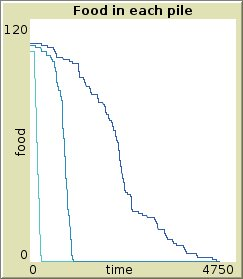
\includegraphics[scale=0.6]{contenu/2antstype.jpg} 
\caption{Proportion de nourriture en fonction du temps}
\label{fig:Tas}
\end{figure}
De plus, notre modèle comprend 4 variables modifiables dont 2 pour la modification de la population. En effet, la variable "Population" nous permet de modifier le nombre de fourmis au total qui sont présentent dans notre fourmilière pendant que la variable "pourcentage" calcul le nombre de fourmis chercheuses en fonction de la population totale (voir les explications de ce choix ici \ref{pourcentage}). De plus, nous sommes dans la capacitée de modifier en direct le pourcentage de diffusion ainsi que le pourcentage d'évaporation des phéromones.
\section{Simulation}
\subsection{Cadre expérimental}
Toutes la partie simulation de ce projet à été effectué avec le logiciel Netlogo 5.1.0 en utilisant le modèle de base fourni. (Wilensky, U. (1997). NetLogo Ants model. http://ccl.northwestern.edu/netlogo/models/Ants. Center for Connected Learning and Computer-Based Modeling, Northwestern University, Evanston, IL.)

Voici les paramètres utilisés :
\begin{figure}[H]
\centering
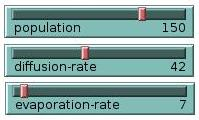
\includegraphics[scale=0.6]{contenu/settings.jpg} 
\caption{Configuration de la simulation}
\label{fig:Tas}
\end{figure}

La population à été déterminée de façon arbitraire, mais telle qu'elle ne soit ni trop basse pour être significative, ni trop haute afin de garder les ressources nécessaires à la modélisation acceptables. Après plusieurs essai, nous avons choisi de garder les paramètres "diffusion-rate" et "evaporation-rate" tel que dans le modèle car ils fournissent une simulation assez plausible : trop de diffusion réduit l'efficacité car la piste laissé est trop large, tandis que trop d'évaporation annule la diffusion. A l'opposé, aucune évaporation est contre productif car l'espace devient saturé de phéromones ce qui revient au même que de ne pas en avoir.

L'univers est un canvas de dimension 81*81 aux bords fermés contenant 1 nid et 3 sources de nourritures de (approximation de cercle de rayon 5) placés spécifiquement.

L'étude des données et leur présentation ont étés effectué avec les outils suivants :
\begin{enumerate}  
\item Python (script) pour le formatage des fichiers .csv
\item Gnuplot pour la représentation des données.
\item R pour l'interprétation mathématique  \ldots 
\item \LaTeX\xspace pour la présentation et le rapport %xspace obligatoire pour l'espacement
\end{enumerate}.

Toutes les simulation et la majeur partie du projet ont étés réalisés sous Ubuntu sur les machine de la Faculté des Sciences de Nice. 


%reference a l'explication des pourcentages
\label{pourcentage}

\subsection{Protocole expérimental}
Pour produire les données permettant de bâtir un modèle nous avons utilisé l'outil BehaviorSpace intégré à Netlogo. Celui ci permet d'exécuter de manière automatiques un nombre déterminé de simulations en faisant varier automatiquement les paramètres voulu.

Afin d'obtenir des mesures les plus objectives possibles nous avons procédé ainsi :
\begin{itemize}  
\item Faire varier la variable "pourcentage" de chercheuse dans la population dans [1;90] par pas de 5, soit 18 runs.
\item Répéter l'expérience précédente pour des sources de nourritures placées à distances  proches, moyenne, et éloignés du nid. Soit 3*18 = 54 simulations retenues.
\item Écrire le nombre de ticks nécessaire à la complétion de la simulation à chaque étape
\item Produire une moyenne des 3 fichiers résultats avec python.
\item Trouver l'équation approximant le mieux nos résultats par régression linéaire avec R
\end{itemize}.

Nous précisons aussi que les simulations ont étés faites consécutivement et non en parallèle dans la configuration de l'outil BehaviorSpace.
\section{Résultats}
Bien que cela semblait évident, nous avons bien pu vérifier que l'ajout de fourmis chercheuses a bien une influence sur l'efficacité de la récolte de nourriture. En effet, plutôt que de chercher au hasard en permanence, les fourmis construisent une trace de phéromones leur permettant de trouver et de se souvenir de l'emplacement du tas de nourriture.

Lorsque nous plaçons les tas de nourriture très proches de la colonie, la durée de ramassage diminue fortement jusqu'à atteindre un minimum local autour de 40\% de fourmis chercheuses avant que la durée ne recommence à augmenter.

\begin{figure}[H]
\centering
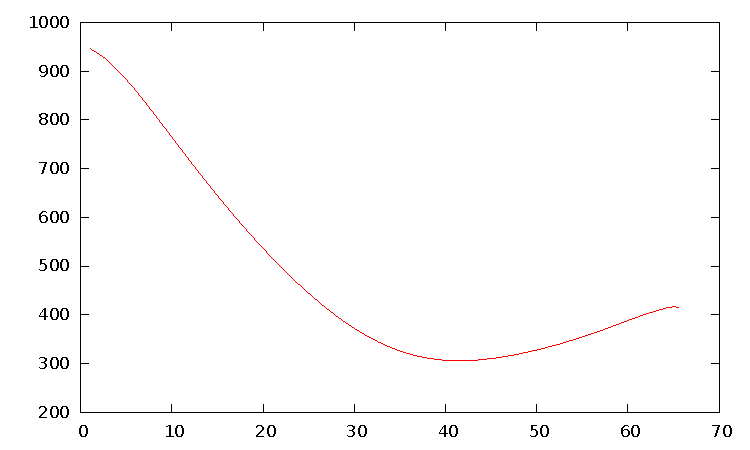
\includegraphics[scale=0.6]{contenu/near.pdf}
\caption{Temps de ramassage en fonction de la proportion de fourmis ramasseuses quand la nourriture est proche}
\label{fig:proche}
\end{figure}

De même, nous observons la même tendance lorsque la nourriture est à distance moyenne et longue de la colonie :

\begin{figure}[H]
\centering
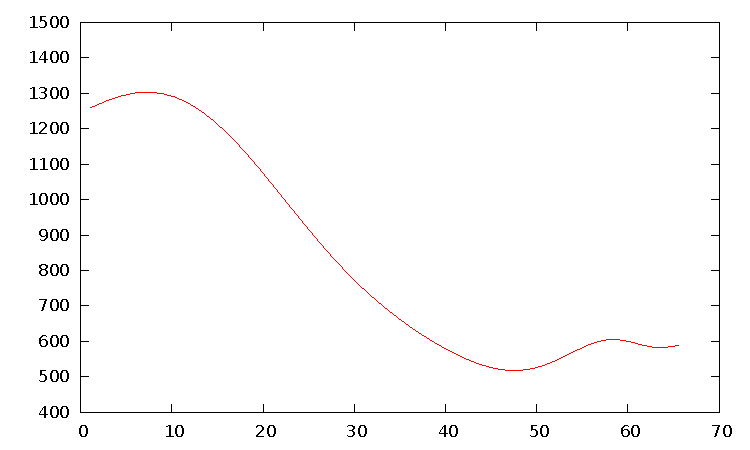
\includegraphics[scale=0.6]{contenu/middle.pdf}
\caption{Temps de ramassage en fonction de la proportion de fourmis ramasseuses quand la nourriture est à distance moyenne}
\label{fig:moyen}
\end{figure}

Dans ce cas, il est important de noter que les points d'inflexion de la courbe sont légèrement décalés vers les hauts pourcentages par rapport à la figure précédente, bien qu'ils remontent ensuite plus fortement.

\begin{figure}[H]
\centering
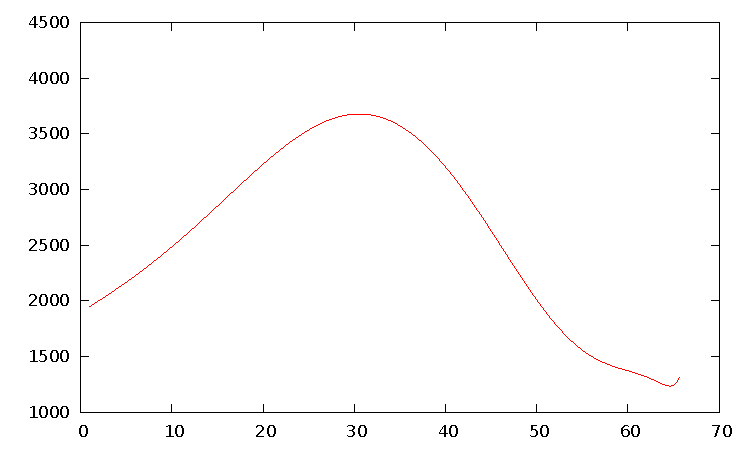
\includegraphics[scale=0.6]{contenu/far.pdf}
\caption{Temps de ramassage en fonction de la proportion de fourmis ramasseuses quand la nourriture est loin}
\label{fig:loin}
\end{figure}

Lorsque les tas de nourriture sont loin, nous pouvons encore émettre les mêmes remarques que précédemment. Les courbes étant très similaires, il semble raisonnable de faire une moyenne afin d'avoir une idée plus générale du comportement des fourmis. Pour chaque pourcentage testé, nous avons donc pris la moyenne de la mesure associée pour chacune des trois distances. Le jeu de données obtenu a ensuite servi à extrapoler par régression polynomiale une expression mathématique nous permettant de donner une estimation du temps de récolte en fonction de la proportion de fourmis chercheuses dans la fourmilière. 

Soient x le pourcentage de fourmis chercheuses et f(x) le temps de récolte :

\begin{math}
 f(x) = 0.0181\cdot x^3 - 2.3204\cdot x^2 + 66.7091\cdot x + 1210.3016
 \end{math}

\begin{figure}[H]
\centering
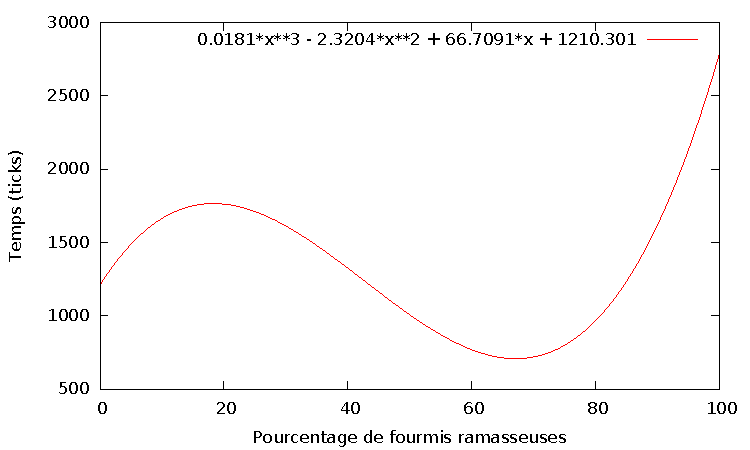
\includegraphics[scale=0.6]{contenu/avg.pdf}
\caption{Temps de ramassage en fonction de la proportion de fourmis ramasseuses}
\label{fig:relation}
\end{figure}

La courbe nous montre que la relation est bien ce qui est attendu : d'abord une augmentation du temps de récolte, puis un minimum autour de 70\% suivi d'une augmentation très rapide.
\section{Discussion}
Il est important de porter un regard critique sur la relation obtenue. En effet, bien qu'elle soit fidèle aux résultats obtenue et observés dans la nature, on suppose qu'il a au moins une ramasseuse puisqu'à 100\% de chercheuses le temps de ramassage, qui devrait être infini, ne l'est pas.

D'autre part, ils aurait été plus rigoureux de faire un moyenne sur un très grand nombre de mesures afin de réduire au maximum l'erreur, le temps ne nous l'a pas permis. 

\section*{Conclusion et perspectives}
Cette étude nous a donc permis d'extraire un modèle mathématique nous donnant une estimation de la durée nécessaire pour ramasser de la nourriture. Le modèle utilisé n'étant pas parfait, il serait intéressant de tester l'efficacité de ce modèle : comment prendre en compte le nombre de tas de nourriture ? Que se passe-t-il lorsqu'il y a des nids rivaux à proximité ? D'autres types de fourmis pour défendre la colonie ou se disputer les sources de nourriture ?
\end{document}
